% Preamble
\documentclass[12pt, a4paper]{report}

% Packages
\usepackage{titlesec,graphicx,tabularx,amsmath,indentfirst,multirow}
\usepackage[T2A] {fontenc}
\usepackage[russian]{babel}
\usepackage[utf8x] {inputenc}
\usepackage[top=2cm, bottom=2cm, left=1.5cm, right=1cm]{geometry}

\titleformat{\section}
{\Large\bfseries} % format
{}                % label
{0pt}             % sep
{\Large}          % before-code

\begin{document}
    \begin{footnotesize}
        \textit{\mbox{Федеральное государственное бюджетное образовательное учреджение высшего профессионального образования}}\\
    \end{footnotesize}

    \begin{tabular}{c c}
        \multirow{4}{*}{
\includegraphics[scale = 0.03]{mgtu.png}}
        & \\
        & \footnotesize\textit{\textbf{\guillemotleftМосковский государственный технический университет имени Н.Э. Баумана\guillemotright}}\\
        & \\
        & \textit{\textbf{(МГТУ им. Н.Э. Баумана)}}\\
        & \\
        & \\
        & \\
        \hline\\
    \end{tabular}

    ФАКУЛЬТЕТ \guillemotleftИнформатика и системы управления\guillemotright\\

    КАФЕДРА \guillemotleft Компьютерные системы и сети\guillemotright\\

    \vfill

    \begin{center}

        \textbf{Отчет}\\
        \bigskip
        \textbf{по домашнему заданию №2}\\
        \bigskip
        \textbf{Дисциплина: Электротехника}\\
        \bigskip
        \textbf{Название лабораторной работы:\\ Анализ электрической цепи переменного тока.}\\
        \bigskip\bigskip
        \textbf{Вариант 10.}\\

        \vfill

        \begin{tabularx}{\textwidth}{X c r}
            Студент гр. ИУ6-35 & $\underset{\text{(Подпись, дата)}}{\makebox[2.0in]{\hrulefill}}$ & Т.Ш. Магомедов\\
            & & \\
            Преподаватель & $\underset{\text{(Подпись, дата)}}{\makebox[2.0in]{\hrulefill}}$ & С.Р. Иванов\\
        \end{tabularx}
        \bigskip\bigskip\bigskip\bigskip\\
        Москва, 2017
    \end{center}
    \thispagestyle{empty} % убрать номер страницы

    \newpage

    \section{\textbf{Задание}}
    \begin{flushleft}
        1. Для приведенного на рисунке варианта схемы получить аналитическое описание коэффициента
        передачи цепи по \textit{Ku(jw)}.\\
        2. Используя полученное описание \textit{Ku(jw)}, вычислить значение модуля коэффициента передачи по
        напряжению и угла сдвига по фазе между выходным и входным напряжением.\\
        3. Пользуясь пакетом прикладных программ EWB Workbench построить \textit{АЧХ} и \textit{ФЧХ}
        анализируемой цепи, а также получить временные диаграммы входного и выходного напряжений.\\
        4. Сопоставить расчетные и экспериментальные данные и сделать необходимые выводы об
        особенностях поведения схемы во временной и частотной областях.\\
    \end{flushleft}
    \bigskip\bigskip\bigskip
    \section{\textbf{Схема цепи}}
    \begin{center}
        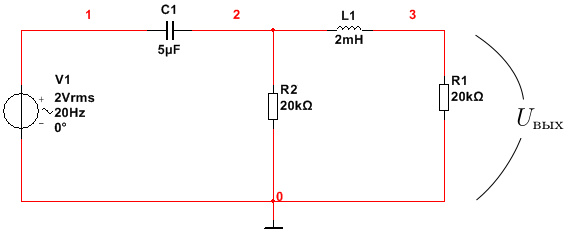
\includegraphics[scale = 3]{photo1.png}\\
        \bigskip\bigskip
        \[ \omega = 2\pi f = 2 \times \pi \times 20 = 125,7 \]
    \end{center}\\
    \section{Найдем сопротивления}
    \[ \dot{Z}_{(R_1,L)} = R_1 + j\omega L \]
    \[ \dot{Z}_{(R_1,R_2,L)} = \frac{R_2(R_1 + j\omega L)}{R_1 + R_2 + j\omega L} \]
    \[ \dot{Z}_{\text{общ}} = \dot{Z}_{(R_1,R_2,L)} + \dot{Z}_{C} = \frac{R_2(R_1 + j\omega L)}{R_1 + R_2 + j\omega L} + \frac{1}{j\omega C} = \frac{R_1 + R_2 + j\omega L + R_{2}j\omega C(R_1 + j\omega L)}{j\omega C(R_1 + R_2 + j\omega L)} \]

    \newpage

    \section{\textbf{1. Коэффициент передачи по напряжению}}
    \begin{itemize}
        $ \dot{K}_U = \dfrac{\dot{U}_{\text{вых}}}{\dot{U}_{\text{вх}}} = \dfrac{I_{R_1}R_1}{V_1} $\\\bigskip
        Пусть ток во всей цепи $I$, тогда: $I_{R_1} = I\dfrac{R_2}{R_1 + R_2 + j\omega L}$\\\bigskip
        При чем $I = \dfrac{V_1}{\dot{Z}_{\text{общ}}} = \dfrac{V_{1}j\omega C(R_1 + R_2 + j\omega L)}{R_1 + R_2 + j\omega L + R_{2}j\omega C(R_1 + j\omega L)}$\\\bigskip
        Тогда $I_{R_1} = \dfrac{V_{1}j\omega C(R_1 + R_2 + j\omega L)}{R_1 + R_2 + j\omega L + R_{2}j\omega C(R_1 + j\omega L)} \times \dfrac{R_2}{R_1 + R_2 + j\omega L} $\\\bigskip
        $I_{R_1} = \dfrac{V_{1}j\omega CR_2}{R_1 + R_2 + j\omega L + R_{2}j\omega C(R_1 + j\omega L)} $\\\bigskip
    \end{itemize}
    \begin{itemize}
        \item Найдем коэффициент передачи по напряжению
    \end{itemize}
    \[ \dot{K}_U = \frac{V_{1}j\omega CR_2}{R_1 + R_2 + j\omega L + R_{2}j\omega C(R_1 + j\omega L)} \times \frac{R_1}{V_1} = \]
    \[ = \frac{R_{1}j\omega CR_2}{R_1 + R_2 + j\omega L + R_{2}j\omega C(R_1 + j\omega L)} = \frac{R_{1}j\omega CR_2}{(R_1 + R_2 - R_{2}\omega^{2}LC) + j(\omega L + R_{1}R_{2}\omega C)} = \]
    \[ = \frac{R_{1}R_{2}j\omega C((R_1 + R_2 - R_{2}\omega^{2}LC) - j(\omega L + R_{1}R_{2}\omega C))}{(R_1 + R_2 - R_{2}\omega^{2}LC)^{2} + (\omega L + R_{1}R_{2}\omega C)^2} \]\bigskip
    \begin{itemize}
        \item Выделим действительную и мнимую часть
    \end{itemize}
    \[ Re[\dot{K}_U] = \dfrac{R_{1}R_{2}\omega^{2} C(L + R_{1}R_{2}C)}{(R_1 + R_2 - R_{2}\omega^{2}LC)^2 + \omega^{2}(L + R_{1}R_{2}C)^2} \]
    \[ Re[\dot{K}_U] = 0,97531 \]
    \[ Im[\dot{K}_U] = \dfrac{R_{1}R_{2}\omega C(R_1 + R_2 - R_{2}\omega^{2}LC)}{(R_1 + R_2 - R_{2}\omega^{2}LC)^2 + \omega^{2}(L + R_{1}R_{2}C)^2} \]
    \[ Im[\dot{K}_U] = 0,15529 \]\bigskip

    \section{\textbf{2. Найдем модуль коэффициента передачи по напряжению}}
    \[ |\dot{K}_{U}| = \sqrt{Re^{2}[\dot{K}_U] + Im^{2}[\dot{K}_U]} = \sqrt{0,97531^{2} + 0,15529^{2}} = 0,98759 \]

    \newpage

    \begin{itemize}
        \item Найдем угол сдвига по фазе
    \end{itemize}
    \[ \varphi = \arctg{\left( \frac{Im[\dot{K}_U]}{Re[\dot{K}_U]} \right)} = \arctg{\left( \frac{\frac{R_{1}R_{2}\omega C(R_1 + R_2 - R_{2}\omega^{2}LC)}{(R_1 + R_2 - R_{2}\omega^{2}LC)^2 + \omega^{2}(L + R_{1}R_{2}C)^2}} {\frac{R_{1}R_{2}\omega^{2} C(L + R_{1}R_{2}C)}{(R_1 + R_2 - R_{2}\omega^{2}LC)^2 + \omega^{2}(L + R_{1}R_{2}C)^2}} \right)} = \arctg{\left( \frac{R_1 + R_2 - R_{2}\omega^{2}LC}{\omega^{2}(L + R_{1}R_{2}C)} \right)}\]\bigskip
    \begin{itemize}
        \item Подставим значения и получим
    \end{itemize}
    \[ \varphi = \arctg(0,15914) = 9,04261 \]\bigskip
    \section{3. АЧХ и ФЧХ}
    \begin{center}
        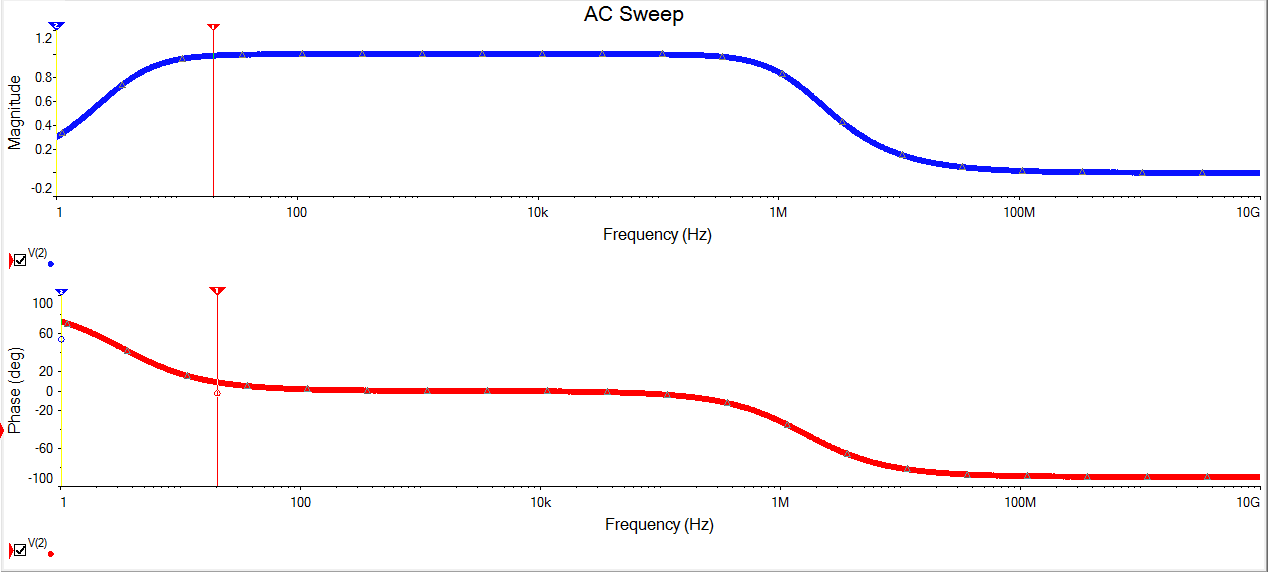
\includegraphics[scale = 0.5]{photo2.png}
    \end{center}\bigskip
    \begin{center}
        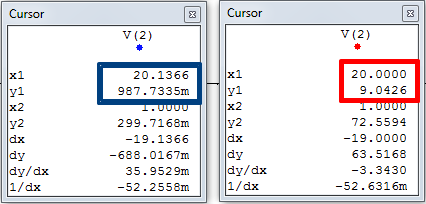
\includegraphics[scale = 1.1]{photo3.png}
    \end{center}

    \newpage

    \begin{itemize}
        \item Временные диаграммы входного и выходного тока и напряжений
    \end{itemize}
    \begin{center}
        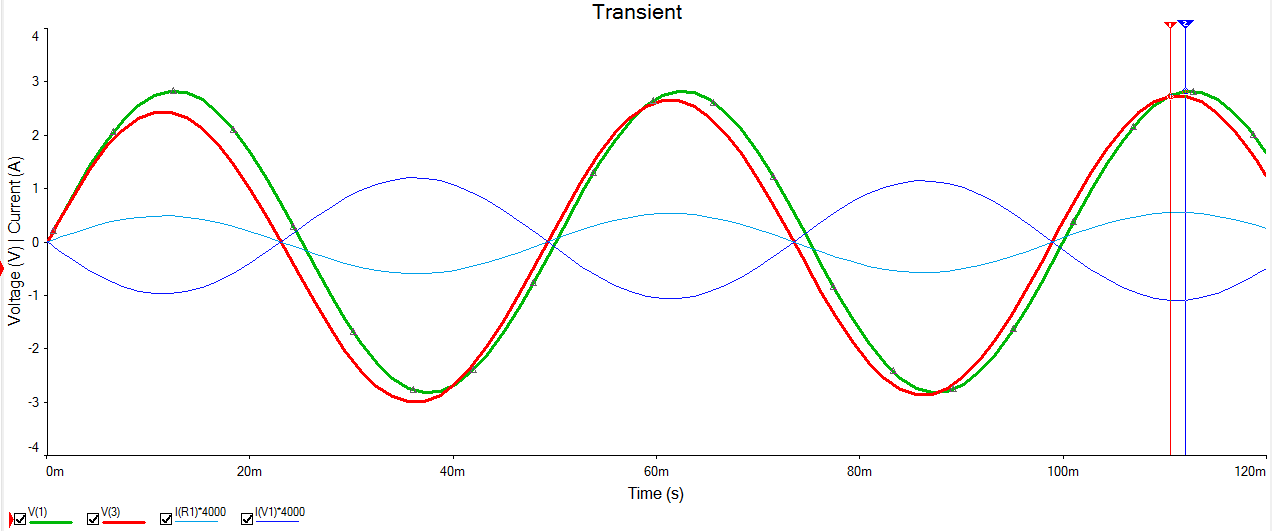
\includegraphics[scale = 0.52]{photo4.png}
    \end{center}
    \begin{center}
        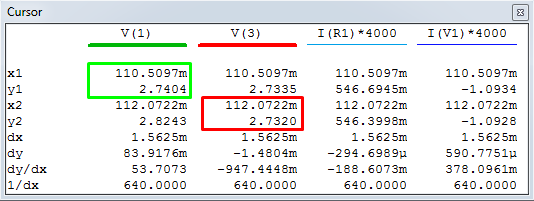
\includegraphics[scale = 1.1]{photo5.png}
    \end{center}\bigskip
    \begin{itemize}
        \item Проведем проверку полученных данных
    \end{itemize}
    \[ |\dot{K}_{U}| = \frac{y_2(V_3)}{y_1(V_1)} = \frac{2,732}{2,7404} = 0,997 \]
    \[ \varphi = \omega \Delta t = 125,7 \times (112,1 - 110,5) \times 0,001 = 0,2 \textit{ рад.} = 11,5 \textit{ град.} \]\bigskip
    \section{4. Выводы}
    \begin{itemize}
        Значение модуля коэффициента передачи по напряжению и значение угла
        сдвига по фазе между выходным и входным ннапряжением примерно совпал со
        значением $y_1$ на \textit{АЧХ} и \textit{ФЧХ} соответственно. Значит, аналитическое описание
        коэффициента передачи цепи по напряжению \textit{Ku(jw)} сделано верно. Неточность
        вызвана вследствие арифметических упрощений при вычислениях.
    \end{itemize}
\end{document}